\subsection{Amphoteric cell}%
\label{sub:some_kind_of_splitting_method_}

An existing H2O electrolysis method which uses an electrolytic cell under alkaline conditions \cite{Zeng2010}, is adapted by adding a membrane and an acidic electrolyte \cite{Lei2019}.

\begin{figure}[H]
	\centering
	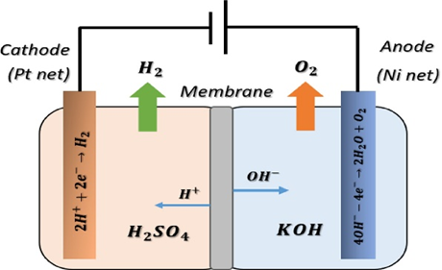
\includegraphics[width=0.4\textwidth]{amphoteric_cell.png}
	\caption{Fig}{Acidic/Alkaline amphoteric electrolytic cell\cite{Lei2019}.}
	\label{fig:amphoteric_cell_diagram}
\end{figure}

An ion-exchange membrane is placed between a \ce{Pt} cathode and an \ce{Ni} anode, this restrains neutralisation between the acidic and alkaline electrolytes.
The \ce{H2SO4} electrolyte provides excess \ce{H+} to react on the surface of the cathode, while the \ce{KOH} electrolyte provides excess \ce{OH-} to react on the surface of the anode.

\begin{align}
	\intertext{\ce{H2} evolution in acidic solution\cite{Lei2019}:} 
	\ce{H3O+ + e- &-> H+ + H2O}\\
	\ce{H3O+ + e- + H^* &-> H2 + H2O}\\
	\intertext{\ce{O2} evolution in alkaline solution\cite{Lei2019}:}
	\ce{OH- &-> OH^* + e-}\\
	\ce{OH- + OH^* &-> O^* + H2O + e-}\\
	\ce{O^* + O^* &-> O2}
\end{align}
(\ce{^*}) - Chemically attaches onto the catalyst.

\ce{H2O} continuously dissociates, the electric potential drives the \ce{H+} into the cathode chamber, and the \ce{OH-} into the anode chamber.
Therefore, the concentration of \ce{H+} and \ce{OH-} in the respective electrolytes is kept high, encouraging the production of \ce{H2} and \ce{O2}.
This results in a lower potential difference for the electrolysis of \ce{H2O}.
Since the experiment took place at a constant current and over a set time, this means that energy consumption was also lower.

So, by using an ion-exchange membrane to separate acidic and alkaline electrolytes, the energy consumption required for the electrolysis of \ce{H2O} was \SI{30}{\percent} less compared to conventional alkaline electrolysis.
If this magnitude of energy efficiency could be achieved on an industrial scale using renewable energy, it would provide a method of producing \ce{H2} from \ce{H2O} without the use of fossil fuels and potentially transform the way we store and release energy.

There is also scope for increased energy efficiency, as increasing temperature led to a lower potential difference for a given \ce{H2} production rate.
This means further research could be undertaken to find the most energy efficient compromise between temperature and potential difference.
Further research could also be undertaken into the composition of the electrodes, and whether there is an alternative combination that is just as effective, but doesn’t require expensive \ce{Pt}.

\subsection{Solar powered steam electrolysis}%
\label{sub:solar_powered_steam_electrolysis}
\cite{Schiller2019}

In this section we discuss steam electrolysis and will look at a case study from Schiller, Lang and Szabo et al\cite{Schiller2019}.
High temperature steam electrolysis operates in the temperature range \SIrange{700}{900}{\celsius}\cite{Schiller2019} and can occur in a solid-oxide electrolysis cell (SOEC); a high operating temperature cell with similar properties to a solid oxide fuel cell, composed of ceramic\cite{Laurencin}.
\begin{figure}[H]
	\centering
	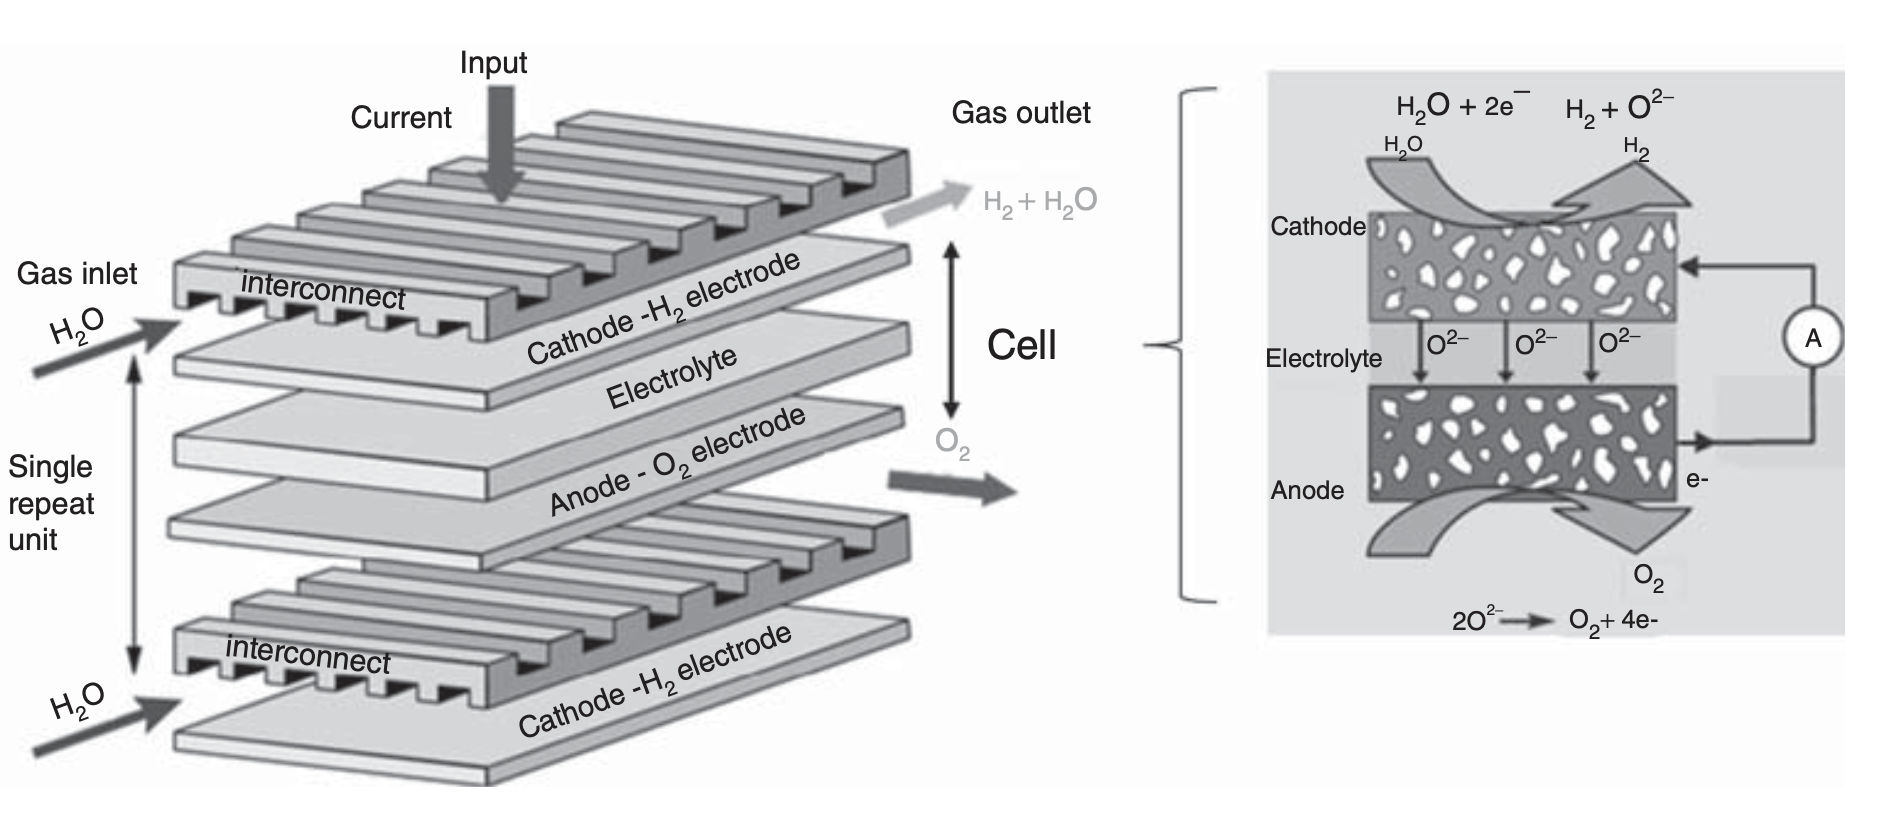
\includegraphics[width=0.4\textwidth]{cf89a71a-2c53-11eb-895f-8c8590753a48.png}
	\caption{The schematic for a single cell of a solid-oxide fuel cell.}
	\label{fig:SE_cell}
\end{figure}
At these temperatures the reaction can proceed faster than at the lower temperatures (\SI{>100}{\celsius}), resulting in a higher electrical efficiency\cite{Schiller2019}.
Overpotential is a major issue with current methods of water electrolysis so overcoming this in systems operating at scale is an important step.

Splitting water in this reaction occurs at two sites; the fuel electrode proceeds via reaction \eqref{eq:SE_fuel_electrode} and the air electrode via \eqref{eq:SE_air_electrode}.\cite{Schiller2019}

\begin{align}
	\ce{H2O + 2e- &-> H2 +O^2-}\label{eq:SE_fuel_electrode}\\
	\ce{O^2- &-> 1/2O2 + 2e-}\label{eq:SE_air_electrode}
.\end{align}

From a thermodynamic perspective the enthalpy required to split water is reduced, as the total enthalpy $\Delta_{r}H$ is significantly lowered by removing the need to supply the enthalpy of vaporisation $\Delta_{\text{vap}}H$, approximately \SI{40.65}{\kilo\joule\per\mole}\cite{Lemmon2017}.
SOECs operating a steam electrolysis reaction have the potential to significantly offset electrical load; the method presented in the paper uses solar energy to superheat water in a steam generator; this is pressurised in an accumulator and fed into the SOEC. 

There are several limitations to this research, while it addresses the possibility of superheating water using solar energy, the experimental set-up uses a solar simulator which is obviously an ideal condition, making this not necessarily geographically suitable.
The SOEC used by the team was a laboratory scale device and could not handle steam mass flow exceeding \SI{0.5}{\kilo\gram\per\hour}, making validating this experiment on a large scale difficult; is solar energy suitable for heating water that can feed a large bank of SOECs, as when lost are kept together they are more thermally efficient.


\subsection{Discussion of water-splitting methods}%
\label{sub:discussion_of_water_splitting_methods}

Acidic/alkaline amphoteric \ce{H2O} electrolytic cells operate below \SI{100}{\celsius}\cite{Lei2019}, whereas solid oxide electrolytic cells (SOEC) operate between \SIrange{700}{1000}{\celsius}\cite{Schiller2019}.
This higher temperature results in faster reactions and a decrease in the Gibbs free enthalpy for \ce{H2O} electrolysis. This results in SOSE requiring less energy per unit volume of \ce{H2}. Additionally, because a large part of the energy required for heating can be provided by solar thermal energy when using SOSE cells, the electrical energy is further lowered. As energy consumption is one of the major problems preventing the uptake of new \ce{H2} productions, this is a clear advantage.

Another advantage of the SOSE is that it uses abundant metals in the electrodes whereas the acidic/alkaline amphoteric cell uses expensive platinum.
Since one of the issues facing new methods of \ce{H2} production is cost this is an important consideration.

Reliability and ease of maintenance are important factors when considering a new process, and SOSE is complex.
It consists of five main components and combines electrical and thermal solar energy sources.
In contrast, the acid/alkaline electrolytic cell is an adaption of an existing technique and is far more simple, with only one main component.

With further refinement SOSE looks to be the most promising method of the two reviewed; it takes the biggest steps in resolving numerous issues facing the use of water electrolysis as a means of producing hydrogen on a large scale.

%Another disadvantage of the acidic/alkaline electrolytic cell is that it depends on an expensive pt electrode, whereas the SOEC uses abundant \ce{Ni}, \ce{La}, \ce{Sr}, \ce{Co}, \ce{Fe}, \ce{Zr} and \ce{Y}.

